\chapter{스핀, 아이소스핀, 색전하와 글루온의 자기 상호작용}

\section{전기역학과의 유추로 이해하는 양자색역학}

양자색역학은 한 강의에서 온전히 전개하기에는 너무 방대한 주제다. 여기서는 더 깊은 수학적 내용보다 기본적인 직관을 얻는 데 초점을 둔다.

양자전기역학은 전자와 광자의 이론이다. 쿨롱 힘의 양자론이기도 하다. 원자핵을 운동이나 내부 구조를 묻지 않는 고정된 전기장 원천으로 취급하면, 양자전기역학은 원자의 이론이 된다.

양자색역학은 쿼크와 글루온에 대해 이와 유사한 역할을 한다. 양자색역학은 입자 자체와 입자 사이의 힘, 그리고 입자들이 이루는 복합체를 기술한다. 이러한 복합체를 \emph{하드론}이라고 한다. 양성자와 중성자는 바리온이다. 이들은 순 쿼크 수, 즉 이와 동등하게 영이 아닌 바리온 수를 가진다. 중간자는 쿼크--반쿼크 조합이다. 바리온과 중간자 모두 글루온도 포함한다.

글루온은 전기적으로 중성이지만 쿼크를 결합하는 장을 제공한다. 이런 점에서 글루온 장은 원자를 결합하는 전자기장과 유사한 역할을 한다.

색전하와 글루온을 도입하기에 앞서 스핀의 수학을 다시 살펴보면 유용하다. 같은 수학이 거의 그대로 \emph{아이소스핀}에서 되풀이되고, 색전하 이론에서도 관련된 구조가 다시 나타난다. 이 구조들의 밑바탕에는 군론이 있지만, 필요한 개념은 각운동량을 통해 설명할 수 있다.

\section{각운동량 다중항}

각운동량 성분은 다음 교환 관계를 만족한다.
\begin{equation}
[L_x,L_y]=i\hbar L_z,
\end{equation}
순환 순서에 따라 다음 관계도 성립한다.
\begin{equation}
[L_y,L_z]=i\hbar L_x,
\qquad
[L_z,L_x]=i\hbar L_y.
\end{equation}
세 성분은 서로 교환하지 않으므로 동시에 모두 측정할 수 없다. 따라서 기술할 때는 한 축을 정해야 한다. 관례적으로 \(z\)축을 택하고, 그 축을 따른 각운동량 성분으로 상태를 표시한다.

이 선택이 자연의 회전 대칭성을 깨뜨리는 것은 아니다. 기록을 위해 한 방향을 정함으로써 기술 방식의 대칭성만 깨진다.

\(z\)성분의 허용값은 양자화되어 있으며 \(\hbar\)만큼씩 차이가 난다. 이 값들을 나열할 때 \(\hbar=1\)로 두면, 스핀 \(\ell\) 다중항은 다음 값을 포함한다.
\begin{equation}
m=\ell,\ell-1,\ldots,-\ell.
\end{equation}
따라서 독립 상태의 수는 다음과 같다.
\begin{equation}
2\ell+1.
\end{equation}

처음 몇 다중항을 직접 적어 보면 다음과 같다.
\begin{align}
\ell=0:&\qquad m=0,\\
\ell=\frac12:&\qquad m=\frac12,-\frac12,\\
\ell=1:&\qquad m=1,0,-1,\\
\ell=\frac32:&\qquad
m=\frac32,\frac12,-\frac12,-\frac32,\\
\ell=2:&\qquad m=2,1,0,-1,-2.
\end{align}

여기서는 반정수 스핀은 페르미온에, 정수 스핀은 보손에 해당한다는 점을 기억하면 된다. 전자는 스핀 \(\tfrac12\) 입자다. 스핀이 0인 입자는 각운동량이 전혀 없다. 광자의 스핀은 1이며, 원자와 원자핵에도 스핀 1인 상태가 있다. 원자와 원자핵은 스핀 \(\tfrac32\)도 가질 수 있으며, 같은 셈법은 더 높은 스핀에도 이어진다.

표기법에서는 전체 스핀과 그 성분을 구별해야 한다. 수 \(\ell\)은 다중항을 나타내며, 가능한 \(z\) 성분의 최댓값이기도 하다. 수 \(m\)는 그 다중항 안의 특정 상태를 나타낸다. 따라서 스핀 1인 대상에는 상태가 세 개 있고, 스핀 \(\tfrac12\)인 대상에는 상태가 두 개 있다.

\section{스핀 1/2 입자 두 개의 결합}

궤도 각운동량은 무시하고 스핀 \(\tfrac12\) 입자 두 개를 생각해 보자. 두 입자의 스핀 곱공간에는 다음 네 기저 상태가 있다.
\begin{equation}
|\uparrow\uparrow\rangle,\qquad
|\uparrow\downarrow\rangle,\qquad
|\downarrow\uparrow\rangle,\qquad
|\downarrow\downarrow\rangle.
\end{equation}
각 상태에 해당하는 \(z\) 성분은 다음과 같다.
\begin{align}
|\uparrow\uparrow\rangle &: m=+1,\\
|\uparrow\downarrow\rangle &: m=0,\\
|\downarrow\uparrow\rangle &: m=0,\\
|\downarrow\downarrow\rangle &: m=-1.
\end{align}

두 스핀이 모두 위를 향하는 상태를 보면 스핀 1 다중항이 반드시 있어야 함을 알 수 있다. \(z\) 성분의 최댓값이 \(+1\)이기 때문이다. 스핀 1 다중항에는 상태가 세 개뿐이다.
\begin{equation}
m=+1,\quad 0,\quad -1.
\end{equation}
하지만 곱공간에는 \(m=0\)인 상태가 서로 독립적으로 두 개 있는 것을 포함해 네 상태가 있다. 이들을 모두 하나의 스핀 1 다중항에 넣을 수는 없다. 남는 상태를 스핀 2로 볼 수도 없다. 스핀 2 다중항에는 상태가 다섯 개 필요하기 때문이다. 따라서 네 곱상태는 스핀 1인 세 상태와 스핀 0인 한 상태로 나뉘어야 한다.

\(m=0\)인 두 기저 상태의 어떤 조합이 스핀 1 다중항에 속할까? 두 입자를 서로 맞바꾸어 보자. 두 스핀이 나란한 상태는 바뀌지 않는다.
\begin{equation}
|\uparrow\uparrow\rangle\longrightarrow|\uparrow\uparrow\rangle,
\qquad
|\downarrow\downarrow\rangle\longrightarrow|\downarrow\downarrow\rangle.
\end{equation}
반면 스핀 곱상태가 서로 바뀐다.
\begin{equation}
|\uparrow\downarrow\rangle
\longleftrightarrow
|\downarrow\uparrow\rangle.
\end{equation}
이 두 상태의 합은 서로 맞바꾸어도 대칭이다.
\begin{equation}
|\uparrow\downarrow\rangle+|\downarrow\uparrow\rangle.
\end{equation}
정규화하려면 \(1/\sqrt2\)를 곱해야 한다.
\begin{equation}
|1,0\rangle
=
\frac{|\uparrow\downarrow\rangle
      +|\downarrow\uparrow\rangle}{\sqrt2}.
\end{equation}

\begin{figure}[h]
\centering
\includegraphics[width=0.78\textwidth]{lecture_02_figure_02.png}
\caption{스핀 1 삼중항의 \(m=0\) 성분을 이루는 대칭 혼합 스핀 조합.}
\lectureframe{00:15:08}
\end{figure}

두 스핀이 나란한 상태와 함께 이 상태는 스핀 1 삼중항을 이룬다.
\begin{align}
|1,+1\rangle &=|\uparrow\uparrow\rangle,\\
|1,0\rangle &=
\frac{|\uparrow\downarrow\rangle
      +|\downarrow\uparrow\rangle}{\sqrt2},\\
|1,-1\rangle &=|\downarrow\downarrow\rangle.
\end{align}
남은 직교 조합에는 마이너스 부호가 붙는다.
\begin{equation}
|0,0\rangle
=
\frac{|\uparrow\downarrow\rangle
      -|\downarrow\uparrow\rangle}{\sqrt2}.
\end{equation}
이 조합은 두 입자를 맞바꾸면 반대칭이 되며, 상태가 하나뿐인 스핀 0 다중항을 이룬다. 따라서
\begin{equation}
\frac12\otimes\frac12=1\oplus0.
\end{equation}

대칭 혼합 스핀 상태는 \(m=0\)이지만, 전체 각운동량이 0인 것은 \emph{아니다}. 이 상태는 스핀 1 삼중항에 속한다. 좌표축을 회전하면 이 상태는 \(m=\pm1\) 상태들과 섞인다. 반대칭 조합만이 \(\ell=0\)을 가진다.

각운동량만 놓고 보면 단일항은 빈 공간과 같다. 에너지나 전하, 다른 양자수는 가질 수 있지만 각운동량은 갖지 않는다.

이 구분은 사고 실험으로 검증할 수 있다. 각운동량 보존을 제외한 모든 보존 법칙을 무시하고, 어떤 두 입자 스핀 상태가 그냥 사라질 수 있는지 물어보자. 두 정렬 상태는 각각 스핀 1 다중항에 속하므로 어느 쪽도 사라질 수 없다. 대칭적인 \(m=0\) 상태도 사라질 수 없다. 그 \(z\)-성분은 사라지지만, 다른 축을 기준으로는 의미 있는 성분을 가지므로 전체 스핀은 여전히 1이다. 각운동량 보존을 위반하지 않고 사라질 수 있는 상태는 반대칭 단일항뿐이다.

\begin{classroomqa}
\audiencequestion{대칭 혼합 스핀 상태를 \(z\)축을 따라 측정하면 \(+1\)이 나올까, 아니면 \(-1\)이 나올까?\lecturetimestamp{00:19:28}}
\lecturerresponse{아니다. \(z\)축을 따라 측정하면 0이 나온다. 그래도 이 상태의 전체 스핀은 1이므로 다른 축을 따라 측정하면 \(+1\) 또는 \(-1\)이 나올 수 있다.}
\end{classroomqa}

\section{스핀 1/2 입자 세 개}

이제 스핀 \(\tfrac12\) 입자 세 개를 결합해 보자. 곱상태의 수는 다음과 같다.
\begin{equation}
2\times2\times2=8
\end{equation}
세 스핀이 모두 위를 향하면 전체 \(z\) 성분은 \(+\tfrac32\)이다. 따라서 스핀 \(\tfrac32\) 다중항이 반드시 있어야 한다. 이 다중항에는 상태가 다음만큼 있다.
\begin{equation}
2\left(\frac32\right)+1=4
\end{equation}

네 상태가 남는다. 이미 \(m=\pm\tfrac32\)인 상태들을 사용했으므로, 이 상태들은 두 번째 스핀 \(\tfrac32\) 다중항을 이룰 수 없다. 남은 상태들의 최대 성분은 \(+\tfrac12\)와 \(-\tfrac12\)뿐이다. 세 개의 반정수 스핀으로 전체 스핀 0을 만들 수도 없다. 그러므로 남은 상태들은 스핀 \(\tfrac12\) 다중항들을 이루어야 한다.

스핀 \(\tfrac12\) 다중항에는 상태가 두 개 있다. 상태 네 개가 남았으므로 서로 다른 스핀 \(\tfrac12\) 다중항이 두 개 있다.
\begin{equation}
\frac12\otimes\frac12\otimes\frac12
=
\frac32\oplus\frac12\oplus\frac12.
\end{equation}
스핀 업과 스핀 다운이라 부르는 두 상태를 업과 다운이라 부르는 두 쿼크 향으로 바꾸면, 이 구조가 다시 나타난다.

\section{내부 스핀으로서의 아이소스핀}

아이소스핀 또는 동위원소 스핀은 보통 스핀에 대응하는 내부 양이다. 보통 스핀은 물리적 공간의 회전과 관련된다. 아이소스핀은 그렇지 않다. 아이소스핀은 내부 수학 공간에서의 변환을 다루며, 그 공간의 기본 상태 두 개를 다음과 같이 정한다.
\begin{equation}
u,\qquad d.
\end{equation}
여기서 \emph{업}과 \emph{다운}은 향을 나타내는 이름일 뿐이다. 보통 공간에서 위나 아래를 가리키는 것은 아니다.

\editorialnote{내부 스핀 공간의 정의에서 이어지는 강입자 질량 규모에 관한 논의로 넘어가는 짧은 전환 부분은 확실하게 복원할 수 없다. 그 부분에서 추가적인 물리적 주장을 추론하지 않는다.}

왜 \(u\)와 \(d\)이 이 유추에 적합할까? 강입자 물리학의 자연스러운 에너지 규모는 수백 MeV 정도다. 전형적인 가벼운 중간자의 질량은 수백 MeV 정도이며, 세 쿼크를 묶어 핵자를 만드는 데 관여하는 에너지도 그 정도 규모다. 이에 비해 보통 원자핵의 결합 에너지는 몇 MeV에 불과하다. 따라서 원자핵 안에서 양성자와 중성자를 묶는 힘은 강입자 내부에서 쿼크를 결합하는 동역학보다 훨씬 작은 에너지 규모에서 다루고 있다.

여섯 쿼크 향 가운데 \(u\)와 \(d\)는 강입자 규모에 비해 가볍다. 무거운 쿼크를 생성하려면 에너지가 더 많이 필요하고, 그런 쿼크를 포함하는 강입자는 더 가벼운 강입자로 붕괴할 수 있다. 따라서 가장 안정한 가벼운 강입자는 업 쿼크와 다운 쿼크로 이루어진다.

다운 쿼크는 업 쿼크보다 무거우며, 여기서 사용하는 추산으로는 질량이 대략 두 배다. 그러나 두 쿼크의 질량은 모두 수백 MeV에 비해 작다. 1차 근사에서는 강입자 규모에서 둘 다 거의 질량이 없는 것으로 취급할 수 있다. 더 중요한 점은 둘의 질량이 거의 같다고 볼 수 있다는 것이다.

이 근사적인 등가성은 대칭성을 낳는다. 업 쿼크와 다운 쿼크를 서로 바꾸어도 강한 상호작용 물리는 거의 변하지 않는다. 양성자,
\begin{equation}
p\sim uud,
\end{equation}
와 중성자,
\begin{equation}
n\sim udd,
\end{equation}
가 가장 간단한 예다. 두 입자는 \(u\)와 \(d\)를 서로 바꾼 차이만 있고, 질량은 매우 비슷하다.

따라서 다음 교환은
\begin{equation}
u\longleftrightarrow d
\end{equation}
수학적으로 다음과 같은 변환으로 취급된다.
\begin{equation}
|\uparrow\rangle\longleftrightarrow|\downarrow\rangle.
\end{equation}
보통 스핀에서는 이 변환이 공간에서 축을 회전하는 것에 해당한다. 아이소스핀에서는 내부 공간에서의 회전이다. 물리적 의미는 다르지만 수학적 구조는 유사하다.

\begin{figure}[h]
\centering
\includegraphics[width=0.80\textwidth]{lecture_02_figure_03.png}
\caption{스핀 \(\tfrac12\) 상태 두 개의 삼중항 및 단일항 분해. 이에 대응하는 아이소스핀 구성을 설명하는 모형이다.}
\lectureframe{00:27:42}
\end{figure}

\emph{아이소}라는 접두사는 \emph{동위원소}에서 유래했다. 예전 핵물리학적 설명에서는 양성자와 중성자를 하나의 내부 이중항을 이루는 두 구성원으로 보았다. 원자핵에서 양성자와 중성자를 맞바꾸면 다른 동위원소가 된다. 이후 쿼크 모형은 이 양성자와 중성자의 교환이 근본적으로 \(u\)와 \(d\)의 교환에서 비롯된다는 점을 설명했다.

\begin{classroomqa}
\audiencequestion{아이소스핀은 쿼크 모형보다 먼저 도입되었나요?\lecturetimestamp{00:30:19}}
\lecturerresponse{그렇다. 아이소스핀은 쿼크가 등장하기 전에 도입되었으며, 역사적으로 하이젠베르크와 관련이 있다. 이후 쿼크 모형은 이를 \(u\) 및 \(d\) 향으로 해석할 근거를 제공했다.}
\end{classroomqa}

아이소스핀은 자연의 정확한 대칭성이 아니다. 업 쿼크와 다운 쿼크의 질량은 정확히 같지 않고, 전하도 서로 다르다.
\begin{equation}
Q(u)=+\frac23,
\qquad
Q(d)=-\frac13.
\end{equation}
질량이 같더라도 전자기력은 여전히 두 쿼크를 구별한다.

작은 강입자계와 원자핵계에서는 강한 상호작용에 비해 전자기 효과가 약하다. 큰 원자핵에서는 전기적 반발이 중요해질 수 있다. 양성자나 중성자, 또는 헬륨과 같은 작은 원자핵에서는 강한 상호작용의 에너지 규모에 비해 전자기 효과가 비교적 작은 보정이다. 따라서 아이소스핀 근사는 다음 두 단계로 이루어진다.

\begin{enumerate}
\item \(u\)--\(d\) 질량 차이를 무시한다.
\item 전자기적으로 서로 구별되는 효과를 끄고 강한 상호작용만 고려한다.
\end{enumerate}

이 근사 안에서는 \(u\)와 \(d\) 사이의 변환이 보통 스핀 대칭성과 수학적으로 유사한 대칭성이 된다.

\section{핵자의 아이소스핀 이중항}

단일 쿼크를 분리해 실험실에서 자유 입자로 조사할 수는 없다. 관측되는 가장 단순한 바리온은 쿼크 세 개로 이루어진다. 따라서 세 스핀의 셈법에 직접 대응하는 아이소스핀의 경우에도 아이소스핀 \(\tfrac12\) 쿼크 세 개가 전체 아이소스핀 \(\tfrac32\) 또는 \(\tfrac12\)를 이룰 수 있다.

전체 아이소스핀이 \(\tfrac12\)인 경우부터 살펴보자. 이러한 다중항에는 상태가 다음만큼 있다.
\begin{equation}
2\left(\frac12\right)+1=2
\end{equation}
이 상태들은 양성자와 중성자다.
\begin{equation}
p\sim uud,
\qquad
n\sim udd.
\end{equation}
두 입자의 전하는 다음과 같다.
\begin{align}
Q(p)
&=\frac23+\frac23-\frac13
=+1,\\
Q(n)
&=\frac23-\frac13-\frac13
=0.
\end{align}
\(u\)와 \(d\)를 맞바꾸면 양성자와 중성자도 서로 바뀐다. 이들은 아이소스핀 \(\tfrac12\) 이중항을 이룬다.

교환 대칭성을 논의할 때는 잠시 쿼크 자리 세 개에 \(1,2,3\)이라는 표지를 붙이자. 이 표지를 고정된 쿼크 위치로 오해해서는 안 된다. 쿼크는 움직인다. 양성자 상태에서 성분을 나타내는 한 가지 도식은 다음과 같다.
\begin{equation}
d_1\bigl(u_2u_3-u_3u_2\bigr).
\end{equation}

\begin{figure}[h]
\centering
\includegraphics[width=0.58\textwidth]{lecture_02_figure_04.png}
\caption{도식적인 양성자 상태에서 반대칭화한 두 \(u\) 쿼크 성분.}
\lectureframe{00:35:43}
\end{figure}

이 식의 목적은 페르미온의 교환 반대칭성을 강조하는 데 있다. 양성자의 완전한 파동함수를 나타내는 식은 아니다. 완전한 상태에는 향, 보통 스핀, 공간 의존성, 그리고------색전하가 함께 들어가야 한다.

\editorialnote{아래첨자는 임시로 붙인 자리 또는 단입자 표지다. 같은 \(u\) 향 상태 두 개가 통상적인 반대칭 아이소스핀 단일항을 이루지는 않는다. 따라서 표시된 성분만으로 아이소스핀이 0이라고 결론 내릴 수 없다. 이 성분은 자리 교환에 대한 반대칭화 단계만 따로 보여 주기 위해 남겨 두었다. 양성자의 전체 아이소스핀은 완전한 세 쿼크 상태에서 결정된다.}

앞서 살펴본 스핀 구성과 제한적으로 비교할 수 있는 점은 양자 상태가 표지의 교환에 대해 대칭 또는 반대칭으로 결합될 수 있다는 것이다. 이 비교만으로는 표시된 \(uu\) 성분이 갖는 아이소스핀을 정할 수 없다.

양성자는 보통 스핀 \(\tfrac12\)과 아이소스핀 \(\tfrac12\)을 모두 가진다. 중성자도 마찬가지다. 이들은 서로 다른 양자수다. 보통 스핀은 물리적 회전과 관련되고, 아이소스핀은 \(u\)--\(d\) 내부 대칭성과 관련된다.

\section{델타 사중항}

가벼운 쿼크 세 개는 전체 아이소스핀 \(\tfrac32\)도 이룰 수 있다. 이렇게 만들어지는 네 상태 다중항은 델타 사중항이다.
\begin{equation}
\begin{aligned}
\Delta^{++}&\sim uuu,
&
\Delta^{+}&\sim uud,
\\
\Delta^{0}&\sim udd,
&
\Delta^{-}&\sim ddd.
\end{aligned}
\end{equation}
델타 상태는 아이소스핀 \(\tfrac32\)뿐 아니라 보통 스핀 \(\tfrac32\)도 가진다. 성분이 최댓값인 상태에서는 보통 스핀 세 개가 모두 같은 방향이고, 아이소스핀 세 개도 모두 같은 방향이다.

\(uud\)와 같은 조성만으로 그 상태가 양성자인지 \(\Delta^+\)인지 알 수는 없다. 같은 향 조성도 전체 스핀과 전체 아이소스핀이 서로 다른 상태로 결합될 수 있다.

\begin{classroomqa}
\audiencequestion{델타 사중항의 \(uud\) 상태와 양성자는 무엇이 다른가요?\lecturetimestamp{00:41:08}}
\lecturerresponse{두 상태는 보통 스핀이 다르다. 양성자의 스핀은 \(\tfrac12\)인 반면 델타 상태의 스핀은 \(\tfrac32\)이다. 쿼크들은 전체 아이소스핀 상태도 서로 다르게 결합되어 있다.}
\end{classroomqa}

\begin{classroomqa}
\audiencequestion{델타 사중항의 가운데 두 상태는 아이소스핀 \(\tfrac12\) 상태인가요?\lecturetimestamp{00:41:52}}
\lecturerresponse{아니다. 이들의 아이소스핀 성분은 \(+\tfrac12\)와 \(-\tfrac12\)이지만, 전체 아이소스핀은 \(\tfrac32\)이다. 전체 아이소스핀이 \(\tfrac32\)인 다중항에는 반드시 성분 상태가 네 개 있다.}
\end{classroomqa}

네 아이소스핀 성분은 다음에 해당한다.
\begin{equation}
I_3=\frac32,\frac12,-\frac12,-\frac32.
\end{equation}
이들의 전하는 다음과 같다.
\begin{align}
Q(\Delta^{++})&=+2,\\
Q(\Delta^{+})&=+1,\\
Q(\Delta^{0})&=0,\\
Q(\Delta^{-})&=-1.
\end{align}
가운데 두 상태의 전하는 양성자와 중성자의 전하와 우연히 같지만, 스핀과 아이소스핀의 결합 방식이 다르므로 서로 다른 상태다.

아이소스핀 대칭성이 근사적으로 성립하므로 네 델타의 질량은 거의 같다. \(u\)--\(d\) 질량 차이는 사중항 안에서 작은 질량 분리만 일으킨다. 델타의 공통 질량 규모는 대략 다음과 같다.
\begin{equation}
m_\Delta\sim1200\,\mathrm{MeV},
\end{equation}
반면 양성자와 중성자의 질량은 다음 값에 가깝다.
\begin{equation}
m_N\sim940\,\mathrm{MeV}.
\end{equation}

\subsection{\texorpdfstring{\(\Delta^{++}\)}{의 붕괴}}

델타 상태의 질량은 핵자와 파이온으로 붕괴하기에 충분히 크다. 다음 붕괴를 생각해 보자.
\begin{equation}
\Delta^{++}\sim uuu.
\end{equation}
구성 입자들이 서로 멀어지는 동안 쿼크--반쿼크 쌍이 생성될 수 있다. \(u\bar u\)를 넣으려 하면 최종 상태에 세 개의 \(u\) 바리온이 남게 되어, 주어진 에너지로 가능한 더 가벼운 붕괴 경로가 되지 못한다. 대신 \(d\bar d\) 쌍을 생성하면 구성 입자들이 다음과 같이 다시 모일 수 있다.
\begin{equation}
uuu+d\bar d
\longrightarrow
uud+u\bar d.
\end{equation}
최종 복합체 두 개는 다음과 같다.
\begin{equation}
uud=p,
\qquad
u\bar d=\pi^+,
\end{equation}
따라서
\begin{equation}
\Delta^{++}\longrightarrow p+\pi^+.
\end{equation}

\begin{figure}[h]
\centering
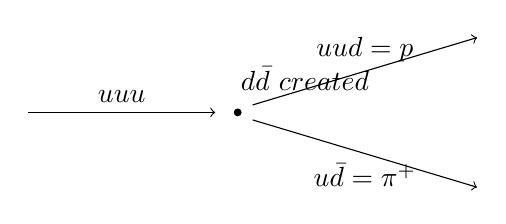
\begin{tikzpicture}[scale=0.95]
\draw[->] (-3,0) -- (-0.5,0) node[midway,above] {$uuu$};
\fill (-0.2,0) circle (1.5pt);
\draw[->] (0,0.1) -- (3,1.0) node[midway,above] {$uud=p$};
\draw[->] (0,-0.1) -- (3,-1.0) node[midway,below] {$u\bar d=\pi^+$};
\node at (0.7,0.45) {$d\bar d\ \text{created}$};
\end{tikzpicture}
\caption{붕괴 \(\Delta^{++}\rightarrow p+\pi^+\)에서 구성 입자들이 다시 모이는 모습.}
\end{figure}

전하 보존은 바로 확인할 수 있다.
\begin{equation}
Q(p)+Q(\pi^+)=1+1=2=Q(\Delta^{++}).
\end{equation}
대략적인 질량 비교로도 이 붕괴가 가능하다.
\begin{equation}
1200\,\mathrm{MeV}
>
940\,\mathrm{MeV}+140\,\mathrm{MeV}.
\end{equation}
최종 상태의 운동에너지로 쓸 에너지도 남는다.

네 델타 상태 모두 양성자 또는 중성자와 파이온으로 붕괴할 수 있다. 이들의 수명은 극히 짧다. 대략적인 크기는 빛이 양성자를 가로지르는 데 걸리는 시간으로 추산할 수 있다.
\begin{equation}
\tau_\Delta
\sim
\frac{10^{-13}\,\mathrm{cm}}
     {10^{10}\,\mathrm{cm/s}}
\sim10^{-23}\,\mathrm{s}.
\end{equation}
그렇지만 입자 충돌에서 생성된 서로 다른 입자로 식별될 만큼은 오래 산다.

\begin{classroomqa}
\audiencequestion{이 구성 성분을 셈할 때 \(u\)와 \(d\) 기호를 적는 순서가 중요한가요?\lecturetimestamp{00:48:49}}
\lecturerresponse{여기서 다루는 목적에는 중요하지 않다. 중요한 것은 향의 조성과 완전한 양자 상태가 결합되는 방식이다.}
\end{classroomqa}

\section{파울리 역설과 색전하의 필요성}

\(\Delta^{++}\)는 모순을 드러낸다. 이 입자는 업 쿼크 세 개로 이루어져 있다. 스핀 \(\tfrac32\) 상태에서는 보통 스핀 세 개가 모두 같은 방향을 향할 수 있다. 세 쿼크가 모두 \(u\)이므로 아이소스핀도 같다. 스핀, 향, 그리고 최저 에너지 공간 상태만으로 전체 상태를 기술한다면, 쿼크 세 개는 같은 상태를 차지하는 동일한 페르미온이 된다. 파울리 배타 원리는 이를 금지한다.

\begin{classroomqa}
\audiencequestion{업 쿼크가 같은 상태를 차지하는 것처럼 보이는데 어떻게 페르미온일 수 있나요?\lecturetimestamp{00:48:58}}
\lecturerresponse{모든 양자수가 똑같을 수는 없다. \(\Delta^{++}\)를 보면 쿼크에는 보통 스핀, 향, 공간 상태 외에 추가 표지가 필요하다. 그 추가 표지가 색전하다.}
\end{classroomqa}

새 표지에는 가능한 값이 세 개 있다.
\begin{equation}
r,\qquad g,\qquad b,
\end{equation}
이를 각각 빨강, 초록, 파랑이라고 부른다. 이 이름들은 눈에 보이는 색과 아무 관련이 없다. 세 가지 내부 상태를 가리키는 임의의 이름이다. 다른 이름을 써도 되며, 중요한 것은 서로 다른 가능성이 세 개라는 점이다.

같은 쿼크 향의 빨강, 초록, 파랑 상태는 질량과 일반적인 관측 성질이 같다. 그래도 이들은 서로 다른 양자 상태다. 따라서 \(\Delta^{++}\)에는 빨강 \(u\) 하나, 초록 \(u\) 하나, 파랑 \(u\) 하나가 들어갈 수 있어 페르미온 세 개가 완전하게 같은 상태를 차지하지 않는다.

여섯 가지 향은 다음과 같다.
\begin{equation}
u,\ d,\ c,\ s,\ t,\ b.
\end{equation}
이 순서는 질량순이 아니다. 업 쿼크가 가장 가볍고 다음은 다운 쿼크다. 참 쿼크는 기묘 쿼크보다 훨씬 무겁고, 톱 쿼크는 바닥 쿼크보다 훨씬 더 무겁다. 각 향은 세 가지 색전하 상태로 존재한다. 따라서 쿼크에는 적어도 다음 두 가지 서로 다른 내부 표지가 있다.
\begin{equation}
\text{flavor}\quad\text{and}\quad\text{color}.
\end{equation}

쿼크들을 위치나 운동량으로 구별할 수는 없었을까? 델타 역설은 최저 에너지 상태에 관한 것이다. 이 상태에서는 에너지와 대칭 성질을 바꾸지 않고 공간 및 운동량 구조만으로 서로 다른 표지를 세 개 만들 수 없다. 빠진 구별은 새로운 내부 자유도여야 한다.

원자물리학에서 스핀이 하는 역할과 유사한 점이 있다. 같은 궤도 상태를 차지하는 것처럼 보이는 전자 두 개도 스핀 상태가 서로 다를 수 있다. 같은 구조로, 향과 보통 스핀, 공간 상태가 같은 쿼크들도 색전하가 다를 수 있다.

\editorialnote{헬륨 분광학, 파울리 원리, 울렌베크와 호우트스미트에 관한 정확한 역사적 경로는 명시적으로 불확실한 것으로 다루었다. 스핀이 정확히 어떤 연대기를 거쳐 발견되었는지 단정하지 않고 유추만 유지한다.}

난부 요이치로는 쿼크에 이 추가 자유도가 필요하다는 점을 알아낸 인물로 알려져 있다. 그 이름과 관계없이 물리적 요점은 같다. 쿼크의 색전하 세 가지가 파울리 모순을 해소한다. 여기서 관련된 배타 원리는 하이젠베르크 불확정성 원리가 아니라 파울리 원리다.

\editorialnote{\emph{색}이라는 이름의 정확한 유래와 이후 역사는 불확실한 것으로 남겨 두었으므로, 여기서는 더 구체적인 연대를 단정하지 않는다. 강의에서 언급된 하이젠베르크 불확정성 원리는 주변의 페르미온 통계 논의에 맞게 파울리 배타 원리로 바로잡았다.}

같은 색전하 개념은 양성자와 중성자에도 적용된다. 이들의 상태는 적힌 향 기호마다 영구히 식별 가능한 색을 하나씩 배정해 구성하는 것이 아니다. 물리적 바리온은 가능한 빨강, 초록, 파랑 배정들의 양자 중첩이며, 적절한 교환 대칭성을 갖도록 결합되어 있다.

\begin{classroomqa}
\audiencequestion{색전하는 직접 측정할 수 있는 보통의 물리적 성질인가요?\lecturetimestamp{00:56:55}}
\lecturerresponse{세 색전하 상태는 질량과 보통의 성질이 같다. 이들의 차이는 허용되는 조합과 충돌 과정에서 관계적으로 드러난다. 색전하를 띤 쿼크를 고립시켜 직접 관찰할 수는 없지만, 실험을 통해 서로 다른 색전하 상태가 세 가지 존재한다는 사실이 확인된다.}
\end{classroomqa}

\begin{classroomqa}
\audiencequestion{색전하는 보존되나요?\lecturetimestamp{00:57:38}}
\lecturerresponse{그렇다. 색전하는 보존된다. 다만 여기서 다루는 관측 가능한 입자는 언제나 색전하 단일항이므로, 조금 낯설게 보이는 보존 법칙이다.}
\end{classroomqa}

\editorialnote{더 정확히 말하면, 점근적 강입자는 색전하 단일항이다. ``색전하가 0''이라는 표현은 빨강, 초록, 파랑을 수치로 더해 얻는 아벨 순전하를 뜻하지 않는다.}

\begin{classroomqa}
\audiencequestion{\(uud\) 양성자에 색전하 세 가지가 정말 모두 필요한가요? \(u\) 쿼크 두 개만 구별하면 충분해 보입니다.\lecturetimestamp{00:57:58}}
\lecturerresponse{그 예에서도 추가적인 구별이 필요하다는 점은 분명하지만, 필요한 표지가 세 가지라는 결론까지 강제하지는 않는다. 보통 스핀과 아이소스핀이 나란한 업 쿼크 세 개로 이루어진 \(\Delta^{++}\)는 서로 다른 표지가 세 개 필요하다는 점을 명확히 보여 준다.}
\end{classroomqa}

이 때문에 델타 입자가 중요한 역할을 했다. 양성자와 중성자는 스핀과 향 대칭성이 더 복잡해 파동함수의 세부 사항에 따라 모순이 가려질 수 있다. \(\Delta^{++}\)에서는 모순이 즉시 드러난다.
\begin{equation}
uuu,\qquad
\uparrow\uparrow\uparrow,
\qquad
\text{one lowest spatial state}.
\end{equation}
세 가지 값을 갖는 새로운 표지가 필요하다. 강입자 충돌 자료도 색전하 상태가 세 가지라는 사실을 독립적으로 확인해 준다.

대칭성 표지는 각 선택지가 단독으로 보았을 때 서로 동등하더라도 의미를 가질 수 있다. 공간에서 정해진 축이 없으면 두 스핀 방향은 물리적으로 동등하다. 다른 물체가 기준축을 제공하면 두 방향의 관계를 알아낼 수 있다. 이와 비슷하게 양성자나 중성자는 아이소스핀 공간에서 방향을 정하며, 다른 상태와 비교하면 내부 방향이 평행한지 반평행한지 알 수 있다. 색전하는 더 미묘하지만, 물리적 의미는 눈에 보이는 색이 아니라 관계와 상관관계, 상호작용 규칙을 통해 드러난다.

파울리 원리를 포기한다고 상상할 수도 있다. 하지만 그러려면 새로운 수학적 틀이 필요하다. 보통의 양자장론은 입자를 페르미온 또는 보손으로 분류하며, 이 문제를 해결하는 것으로 확립된 제3의 선택지는 없다. 양자색역학은 쿼크의 페르미온 성질을 유지하면서 색전하를 도입한다.

\begin{classroomqa}
\audiencequestion{파울리 원리가 요구하는 숨은 구별에 대응하는 관측량은 무엇인가요?\lecturetimestamp{01:01:08}}
\lecturerresponse{이 질문은 익숙한 위치, 운동량, 아이소스핀 관측량보다 훨씬 미묘하다. 완전한 답을 얻으려면 색전하 동역학을 더 살펴봐야 하므로 여기서는 뒤로 미룬다.}
\end{classroomqa}

\begin{classroomqa}
\audiencequestion{강입자의 스핀 배정을 통해 쿼크가 페르미온이라는 사실을 추론했나요?\lecturetimestamp{01:01:43}}
\lecturerresponse{그렇다.}
\end{classroomqa}

\editorialnote{앞의 청중 질문 두 개는 표현의 일부가 명확하지 않다. 질문의 주제와 짧은 답변은 분명하지만, 더 상세한 문구를 추론하지는 않는다.}

\begin{classroomqa}
\audiencequestion{양성자 안의 특정 쿼크에 특정 색전하를 어떻게 배정하나요?\lecturetimestamp{01:01:55}}
\lecturerresponse{영구히 식별 가능한 구성 입자에 고정된 색전하를 배정하지는 않는다. 양성자는 가능한 모든 빨강, 초록, 파랑 배정의 양자 중첩이며, 스핀, 향, 공간, 색전하 성분이 적절하게 대칭화되거나 반대칭화되어 있다. \(\Delta^{++}\)는 스핀과 향이 나란한 구조를 통해 완전한 양성자 파동함수 없이도 색전하가 필요함을 드러내므로 유용하다.}
\end{classroomqa}

양자색역학에서 색전하가 하는 역할은 전기역학에서 전하가 하는 역할과 같다. 상호작용을 좌우하는 양자수다. 양자색역학은 강입자 충돌의 실험 자료를 매우 정확하게 설명한다. 이 틀의 궁극적인 정당성은 그 예측이 실험과 일치한다는 데 있다.

\section{광자와 글루온}

쿼크는 QCD의 페르미온 물질 입자로, 이런 제한된 측면에서는 QED의 전자와 유사하다. 쿼크를 묶어 두는 것은 무엇일까?

전기역학에서 전자는 전자기장의 원천이다. 입자 관점에서 보면 전자는 광자를 방출하고 흡수하며, 광자 교환으로 전하를 띤 입자 사이에 힘이 생긴다. 이와 마찬가지로 쿼크는 글루온장의 원천이며 글루온을 방출하고 흡수할 수 있다.

글루온은 몇 가지 중요한 측면에서 광자와 비슷하다. 글루온은 질량이 없는 스핀 1 입자이며, 광자와 비슷한 편광 상태를 가진다. 운동량과 편광은 일반적인 동역학적 성질이다. 결정적인 차이는 글루온이 색 정보를 지니므로 서로 상호작용한다는 점이다.

광자는 전하를 띠지 않는다. QED의 기본 수준에서는 광자 하나가 다른 광자를 방출하지 않으며, 두 빛줄기는 서로 상호작용하지 않고 지나간다. 전자 고리가 관여하는 더 높은 차수의 광자-광자 상호작용도 있지만, 이는 직접적인 광자 자기결합이 아니라 부차적인 효과다. 진공에서 기본 QED 꼭짓점은 전자가 광자를 방출하거나 흡수하는 과정뿐이다.

\begin{figure}[h]
\centering
\begin{tikzpicture}[scale=1.0]
\draw[->] (-2,-1) -- (0,0);
\draw[->] (0,0) -- (2,-1);
\draw[smooth] plot coordinates {
(0,0) (0.16,0.27) (0.32,0.23) (0.48,0.52)
(0.64,0.48) (0.80,0.77) (0.96,0.73)
(1.12,1.02) (1.28,0.98) (1.44,1.27)
(1.60,1.23) (1.76,1.52)
};
\node at (-1.25,-0.75) {$e^-$};
\node at (1.25,-0.75) {$e^-$};
\node at (1.95,1.62) {$\gamma$};
\fill (0,0) circle (1.5pt);
\end{tikzpicture}
\caption{기본 QED 꼭짓점: 전자가 광자를 방출하거나 흡수한다.}
\end{figure}

페르미온 선의 방향을 뒤집으면 전자에 대한 해석이 양전자에 대한 해석으로 바뀐다. 방출, 흡수, 그리고 교차된 양전자 과정은 모두 이 하나의 꼭짓점을 재배열한 것이다.

계산을 간편하게 하려고 광자가 전자--양전자 쌍의 성질 일부를 가진다고 가정해 볼 수 있다. 이 쌍은 전기적으로 중성이며, 전자와 양전자의 스핀이 나란히 정렬되면 총스핀 1을 이룰 수 있다. 필요한 에너지와 운동량을 외부 상호작용이 공급하면 광자는 전자--양전자 쌍을 만들 수 있다. 그렇다고 광자가 문자 그대로 전자와 양전자로 이루어졌다는 뜻은 아니다. 이 가상 쌍 그림은 QED 자체에는 별 도움이 되지 않지만, 색에 대응하는 그림은 QCD에서 유용하다.

\section{글루온의 색--반색 표기}

쿼크의 세 가지 색 상태를 열벡터로 나타내자:
\begin{equation}
q=
\begin{pmatrix}
r\\
g\\
b
\end{pmatrix}.
\end{equation}
이에 대응하는 반쿼크 표기는 행벡터로 나타내자:
\begin{equation}
\bar q=
\begin{pmatrix}
\bar r&\bar g&\bar b
\end{pmatrix}.
\end{equation}

글루온은 쿼크--반쿼크 결합 상태가 아니다. 그래도 색을 계산할 때는 색 하나와 반색 하나를 지닌 것처럼 다룰 수 있다. 따라서 가능한 표기를 다음과 같이 배열할 수 있다.
\begin{equation}
\begin{pmatrix}
r\bar r&r\bar g&r\bar b\\
g\bar r&g\bar g&g\bar b\\
b\bar r&b\bar g&b\bar b
\end{pmatrix}.
\end{equation}
처음 보면 조합이 아홉 개로 보인다.

\begin{classroomqa}
\audiencequestion{대각선의 색--반색 항목은 서로 구별되지 않나요?\lecturetimestamp{01:13:37}}
\lecturerresponse{그렇지는 않습니다. 대각선 항목은 서로 다릅니다. 다만 그 항목들의 합은 독립적인 양자 상태가 아닙니다.}
\end{classroomqa}

실제로 독립적인 글루온 상태는 여덟 개뿐이다. 세 대각선 표기가 서로 구별되지 않는 것은 아니지만, 다음과 같은 특정 대각선 합은
\begin{equation}
r\bar r+g\bar g+b\bar b
\end{equation}
QCD의 독립적인 글루온을 하나 더 이루지 않는다. 이처럼 상태 수가 줄어드는 자세한 설명은 뒤로 미루자. 지금 다룰 색 흐름 논의에서는 겉보기에 아홉 개인 표기를 사용하되, 대각선 조합 하나가 빠진다는 점을 기억하면 편리하다.

\section{쿼크--글루온 꼭짓점}

쿼크는 글루온을 방출한 뒤 같은 색으로 남을 수도, 다른 색으로 바뀔 수도 있다. 색 \(a\)인 쿼크가 들어와 색 \(b\)인 쿼크가 나가면, 방출된 글루온의 계산용 표기는 \(a\bar b\)이다:
\begin{equation}
a\longrightarrow b+(a\bar b).
\end{equation}
예를 들면,
\begin{equation}
r\longrightarrow g+(r\bar g).
\end{equation}
빨간색 선은 글루온 안으로 이어지고, 초록색 선은 나가는 쿼크를 따라 이어진 뒤 글루온 안에서 반초록색 선으로 방향이 뒤집힌다.

쿼크의 색이 바뀌지 않아도 된다. 같은 규칙에 따라 다음 과정도 가능하다.
\begin{equation}
r\longrightarrow r+(r\bar r),
\end{equation}
또는
\begin{equation}
r\longrightarrow b+(r\bar b).
\end{equation}

\begin{figure}[h]
\centering
\begin{tikzpicture}[scale=1.0]
\draw[->] (-2,-0.8) -- (0,0) node[midway,above] {$r$};
\draw[->] (0,0) -- (2,0.9) node[midway,above] {$g$};
\draw[smooth] plot coordinates {
(0,0) (0.20,-0.23) (0.40,-0.17) (0.60,-0.46)
(0.80,-0.40) (1.00,-0.69) (1.20,-0.63)
(1.40,-0.92) (1.60,-0.86) (1.80,-1.15)
(2.00,-1.09)
};
\node at (2.35,-1.12) {$r\bar g$};
\fill (0,0) circle (1.5pt);
\end{tikzpicture}
\caption{빨간 쿼크가 글루온 \(r\bar g\)을 방출하면서 초록 쿼크로 바뀐다.}
\end{figure}

이것은 QCD를 이루는 기본 구성 요소 하나다.

\begin{classroomqa}
\audiencequestion{쿼크의 색이 바뀔 때만 글루온이 방출될 수 있나요?\lecturetimestamp{01:17:15}}
\lecturerresponse{아닙니다. 나가는 쿼크는 들어온 쿼크와 같은 색일 수도, 다른 색일 수도 있습니다. 어느 경우든 방출된 글루온의 색--반색 표기가 색 선을 끊김 없이 이어 준다.}
\end{classroomqa}

\section{세 글루온 꼭짓점}

QCD에는 QED에 기본적인 대응물이 없는 또 다른 기본 상호작용이 있다. 글루온은 다른 글루온과 직접 상호작용할 수 있다.

\(r\bar b\) 글루온에서 시작하자. 색 흐름으로 보면 이 글루온은 다음과 같이 분리될 수 있다.
\begin{equation}
r\bar b
\longrightarrow
r\bar g+g\bar b.
\end{equation}
빨간색 선은 \(r\bar g\)으로 이어지고, 반파란색 선은 \(g\bar b\)로 이어지며, 초록색-반초록색 쌍은 나가는 두 글루온을 연결한다. 이렇게 세 글루온 꼭짓점이 만들어진다.

\begin{figure}[h]
\centering
\begin{tikzpicture}[scale=1.0]
\draw[smooth] plot coordinates {
(-2,0) (-1.80,0.12) (-1.60,-0.02) (-1.40,0.12)
(-1.20,-0.02) (-1.00,0.12) (-0.80,-0.02)
(-0.60,0.12) (-0.40,-0.02) (-0.20,0.12) (0,0)
};
\draw[smooth] plot coordinates {
(0,0) (0.20,0.27) (0.40,0.21) (0.60,0.50)
(0.80,0.44) (1.00,0.73) (1.20,0.67)
(1.40,0.96) (1.60,0.90) (1.80,1.19) (2.00,1.13)
};
\draw[smooth] plot coordinates {
(0,0) (0.20,-0.27) (0.40,-0.21) (0.60,-0.50)
(0.80,-0.44) (1.00,-0.73) (1.20,-0.67)
(1.40,-0.96) (1.60,-0.90) (1.80,-1.19) (2.00,-1.13)
};
\node at (-2.45,0) {$r\bar b$};
\node at (2.45,1.18) {$r\bar g$};
\node at (2.45,-1.18) {$g\bar b$};
\fill (0,0) circle (1.5pt);
\end{tikzpicture}
\caption{세 글루온의 색 흐름: \(r\bar b\rightarrow r\bar g+g\bar b\).}
\end{figure}

가능한 조합을 하나하나 외울 필요는 없다. 도표에서 각 색 선을 따라가면 된다. 페르미온 선의 시간 방향이 뒤집히면 이에 해당하는 반입자 선이나 반색 선으로 해석하면 된다.

\section{글루온 교환과 힘}

광자가 전하를 띤 입자 사이에서 교환되어 전자기력을 일으키듯, 글루온도 교환을 통해 힘을 일으킨다.

예를 들어, 파란 쿼크와 반파란 반쿼크가 \(g\bar b\) 글루온을 교환하면 초록 쿼크와 반초록 반쿼크로 바뀔 수 있다. 두 꼭짓점을 모두 만족하는 색 흐름 표기는 다음과 같다.\footnote{순 색 변화 \(b+\bar b\longrightarrow g+\bar g\)는 명확하지만, 국소적인 색 표기는 여러 차례 수정된다. 교환되는 표기 \(g\bar b\)는 두 꼭짓점 모두에서 색 흐름이 이어지도록 요구해 재구성한다.}
\begin{equation}
b+\bar b
\longrightarrow
g+\bar g.
\end{equation}
반쿼크 꼭짓점에서는
\begin{equation}
\bar b\longrightarrow\bar g+(g\bar b),
\end{equation}
쿼크 꼭짓점에서는
\begin{equation}
b+(g\bar b)\longrightarrow g.
\end{equation}
교환된 글루온은 한 페르미온 선에서 다른 선으로 색 변화를 전달한다.

\begin{figure}[h]
\centering
\begin{tikzpicture}[scale=1.0]
\draw[->] (-1.8,0) -- (-1.8,-1.8) node[midway,left] {$\bar b$};
\draw[->] (-1.8,1.8) -- (-1.8,0) node[midway,left] {$\bar g$};
\draw[->] (1.8,-1.8) -- (1.8,0) node[midway,right] {$b$};
\draw[->] (1.8,0) -- (1.8,1.8) node[midway,right] {$g$};
\draw[smooth] plot coordinates {
(-1.8,0) (-1.50,0.13) (-1.20,-0.03) (-0.90,0.13)
(-0.60,-0.03) (-0.30,0.13) (0,-0.03)
(0.30,0.13) (0.60,-0.03) (0.90,0.13)
(1.20,-0.03) (1.50,0.13) (1.8,0)
};
\node at (0,0.42) {$g\bar b$};
\fill (-1.8,0) circle (1.5pt);
\fill (1.8,0) circle (1.5pt);
\end{tikzpicture}
\caption{\(g\bar b\) 글루온의 교환으로 파란색--반파란색 쌍이 초록색--반초록색 쌍으로 바뀐다. 반쿼크 화살표는 시간 증가 방향의 반대를 가리킨다.}
\end{figure}

같은 상호작용으로 글루온 사이에도 힘이 작용할 수 있다. 일관된 한 가지 구현은 다음과 같다.\footnote{강의에서는 글루온 사이의 글루온 교환과 선을 따라가는 규칙을 설명하지만, 도표의 국소 표기는 여러 번 수정된다. 제시된 표기는 최종 규칙에 부합하는 한 가지 일관된 구현이며, 중간에 나온 모든 표기를 확실하게 옮긴 것은 아니다.}
\begin{equation}
(r\bar b)+(b\bar r)
\longrightarrow
(r\bar g)+(g\bar r),
\end{equation}
외부의 두 글루온 사이에서 \(g\bar b\) 글루온이 교환된다:
\begin{align}
r\bar b&\longrightarrow r\bar g+g\bar b,\\
b\bar r+g\bar b&\longrightarrow g\bar r.
\end{align}

\begin{figure}[h]
\centering
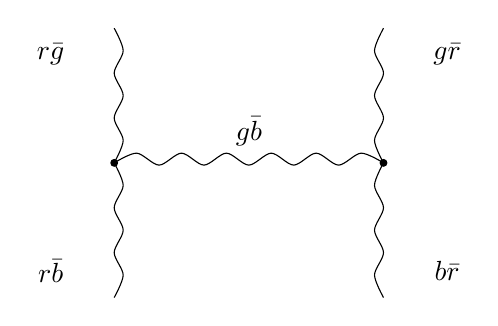
\begin{tikzpicture}[scale=0.95]
\draw[smooth] plot coordinates {
(-1.8,-1.8) (-1.68,-1.50) (-1.80,-1.20) (-1.68,-0.90)
(-1.80,-0.60) (-1.68,-0.30) (-1.8,0)
};
\draw[smooth] plot coordinates {
(-1.8,0) (-1.68,0.30) (-1.80,0.60) (-1.68,0.90)
(-1.80,1.20) (-1.68,1.50) (-1.8,1.8)
};
\draw[smooth] plot coordinates {
(1.8,-1.8) (1.68,-1.50) (1.80,-1.20) (1.68,-0.90)
(1.80,-0.60) (1.68,-0.30) (1.8,0)
};
\draw[smooth] plot coordinates {
(1.8,0) (1.68,0.30) (1.80,0.60) (1.68,0.90)
(1.80,1.20) (1.68,1.50) (1.8,1.8)
};
\draw[smooth] plot coordinates {
(-1.8,0) (-1.50,0.13) (-1.20,-0.03) (-0.90,0.13)
(-0.60,-0.03) (-0.30,0.13) (0,-0.03)
(0.30,0.13) (0.60,-0.03) (0.90,0.13)
(1.20,-0.03) (1.50,0.13) (1.8,0)
};
\node at (-2.65,-1.45) {$r\bar b$};
\node at (-2.65,1.45) {$r\bar g$};
\node at (2.65,-1.45) {$b\bar r$};
\node at (2.65,1.45) {$g\bar r$};
\node at (0,0.42) {$g\bar b$};
\fill (-1.8,0) circle (1.5pt);
\fill (1.8,0) circle (1.5pt);
\end{tikzpicture}
\caption{두 글루온 사이에서 \(g\bar b\) 글루온이 교환되며, 각 색 선과 반색 선은 꼭짓점을 지나며 끊김 없이 이어진다.}
\end{figure}

\section{글루온 자기상호작용과 비선형 장}

글루온 자기상호작용은 QCD의 성격을 바꾼다. 쿼크는 글루온을 교환해 결합하고 강입자를 형성할 수 있으며, 글루온도 글루온을 교환해 결합할 수 있다. 따라서 QCD에는 쿼크 없이 글루온 자유도만으로 이루어진 복합 입자가 존재할 수 있다. QED에는 광자만으로 이루어진 이에 대응하는 기본 결합 상태가 없다.

장으로 표현해도 같은 결론에 이른다. 진공에서는 기본 수준에서 두 전자기파가 서로 지나간다. 두 글루온파는 서로 상호작용하며 변형시킨다. 글루온장 하나의 배치에서도 서로 다른 부분들이 서로 힘을 가할 수 있다. 따라서 글루온장은 비선형이다.

\begin{classroomqa}
\audiencequestion{도표 양쪽에 빨강, 초록, 파랑 표기가 같은 개수로 나타나야 하나요?\lecturetimestamp{01:24:59}}
\lecturerresponse{실용적인 규칙은 도표에서 모든 색 선을 따라가는 것이다. 그렇게 이어지는 것이 색 보존이다. 페르미온 선이 시간상 되돌아가면 표기는 이에 해당하는 반입자 또는 반색 표기로 바뀐다.}
\end{classroomqa}

\begin{classroomqa}
\audiencequestion{도표의 첫 번째 버전에 있는 색과 반색 표기는 모두 일관성이 있나요?\lecturetimestamp{01:26:00}}
\lecturerresponse{아닙니다. 여러 표기를 고쳐야 합니다. 일관된 표기에서는 빨간색, 반파란색, 초록색 선이 각각 꼭짓점을 지나 이어지며, 뒤집힌 페르미온 화살표는 반입자로 해석합니다.}
\end{classroomqa}

\begin{classroomqa}
\audiencequestion{중간 글루온 선을 쿼크--반쿼크 쌍으로 취급하나요?\lecturetimestamp{01:27:58}}
\lecturerresponse{색을 계산할 때만 그렇게 취급합니다. 글루온은 문자 그대로 쿼크--반쿼크 복합체가 아니지만, 이에 해당하는 색과 반색 성질을 지닙니다.}
\end{classroomqa}

이 단계에서 기본 규칙은 간단히 정리할 수 있다:

\begin{itemize}
\item 쿼크는 글루온을 방출하고 흡수한다;
\item 글루온은 다른 글루온과 직접 상호작용한다;
\item 모든 색 선과 반색 선은 꼭짓점을 지나 이어져야 한다;
\item 페르미온 선의 시간 방향을 뒤집으면 이에 해당하는 반입자 선으로 바뀐다.
\end{itemize}

\begin{classroomqa}
\audiencequestion{이렇게 색--반색 선으로 나타내도 글루온은 여전히 질량이 없나요?\lecturetimestamp{01:28:13}}
\lecturerresponse{그렇습니다. 글루온은 질량이 없습니다. 이어지는 설명은 강입자 안의 쿼크에 부여하는 질량이 무엇을 뜻하는지에 관한 단서다.}
\end{classroomqa}

이어서 가둠과 강입자의 구조를 살펴본다. 왜 고립된 색은 관측되지 않으며, 쿼크와 글루온은 복합 입자 안에서 어떻게 조직되는가? 먼저 구성 쿼크의 질량이 무엇을 뜻하는지 분명히 해 두는 것이 유용하다.

\section{쿼크 질량의 탐사 척도와 의미}

질량이 \(m\)인 작은 물체를 부드럽게 변형되는 재료에 붙여 놓았다고 생각해 보자---늘어뜨린 껌 조각이면 된다. 아주 약한 힘을 매우 천천히 가해 부드러운 재료가 반응할 시간을 주고 전체 계가 함께 움직이도록 한다. 그러면 측정되는 관성은 작은 물체와 거기에 붙은 재료의 관성의 합이다.

이제 작은 물체를 매우 높은 주파수로 흔들어 보자. 부드러운 재료는 빠른 움직임을 따라갈 시간이 없다. 작은 중심부가 반응하는 동안 재료는 거의 정지해 있다. 따라서 측정되는 고주파 관성은 오히려 \(m\) 자체의 관성에 더 가깝다.

\begin{figure}[h]
\centering
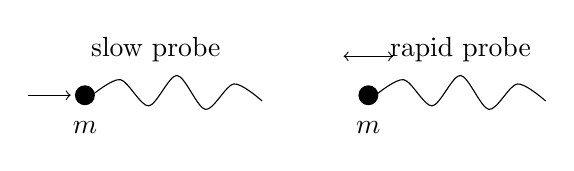
\begin{tikzpicture}[scale=0.9]
\fill (-3,0) circle (4pt);
\node at (-3,-0.45) {$m$};
\draw[smooth] plot coordinates {
(-2.9,0) (-2.5,0.22) (-2.1,-0.15) (-1.7,0.28)
(-1.3,-0.20) (-0.9,0.16) (-0.5,-0.08)
};
\draw[->] (-3.8,0) -- (-3.2,0);
\node at (-2.0,0.65) {slow probe};

\fill (1.0,0) circle (4pt);
\node at (1.0,-0.45) {$m$};
\draw[smooth] plot coordinates {
(1.1,0) (1.5,0.22) (1.9,-0.15) (2.3,0.28)
(2.7,-0.20) (3.1,0.16) (3.5,-0.08)
};
\draw[<->] (0.65,0.55) -- (1.35,0.55);
\node at (2.3,0.65) {rapid probe};
\end{tikzpicture}
\caption{느린 탐사에서는 중심부와 부드러운 부착물이 함께 움직이는 반면, 빠른 탐사에서는 처음에 주로 중심부의 반응을 측정한다.}
\end{figure}

이것은 고전적인 비유다. 주파수에 따라 계의 서로 다른 부분이 참여할 시간이 달라지므로, 가해진 힘의 주파수에 따라 추론되는 질량이 달라진다.

강입자 안의 쿼크는 강하게 상호작용하는 글루온 물질과 다른 구성 입자들로 둘러싸여 있다. 쿼크를 아주 천천히 당길 수 있다면 강입자 전체가 반응할 것이다. 그때 마주치는 관성은 핵자 질량 정도가 된다.
\begin{equation}
m_N\sim930\text{--}940\,\mathrm{MeV}.
\end{equation}
쿼크를 세게 때려 매우 짧은 시간 동안 탐사하면, 처음 나타나는 반응은 가벼운 쿼크에 관례적으로 부여하는 훨씬 작은 질량 매개변수와 관련된다. 대략
\begin{equation}
m_{u,d}\sim5\text{--}10\,\mathrm{MeV}
\end{equation}
여기서 사용하는 추정값은 이렇다.

따라서 ``쿼크의 질량''이라는 말에는 탐사의 척도를 명시해야 한다. 약하고 저주파인 교란은 크기가 큰 복합 입자를 움직이고, 강하고 고주파인 교란은 처음에 훨씬 작은 부분을 분해해 측정한다. 이 비유가 재규격화를 유도하는 것은 아니지만, 입자를 기술하는 데 쓰이는 매개변수가 측정에 사용되는 상호작용의 주파수와 파장에 따라 달라지는 이유를 이해하는 데 도움이 된다. 이렇게 척도에 따라 달라지는 매개변수를 달리는 매개변수 또는 달리는 상수라고 부른다.

\begin{classroomqa}
\audiencequestion{주파수에 따라 달라지는 이 질량은 \(\Delta x\,\Delta t\) 같은 불확정성 관계를 다시 말한 것뿐인가요?\lecturetimestamp{01:33:32}}
\lecturerresponse{아닙니다. 이 예는 고전적 현상만으로도 성립한다. 부드러운 물체에 붙은 작은 질량은 빠른 힘과 느린 힘에 서로 다르게 가속된다. 힘이 빠를 때와 느릴 때 반응할 시간이 있는 부착물의 양이 다르기 때문이다.}
\end{classroomqa}

\begin{classroomqa}
\audiencequestion{전자 전하를 앞서 논의할 때도 이런 종류의 척도 의존성이 있었나요?\lecturetimestamp{01:34:04}}
\lecturerresponse{그렇습니다. 입자를 기술하는 데 쓰이는 매개변수는 탐사에 사용하는 상호작용의 주파수와 파장에 따라 달라진다는 것이 일반적인 교훈이다. 이런 매개변수를 달리는 상수라고 부른다.}
\end{classroomqa}

\begin{classroomqa}
\audiencequestion{쿼크에 부여하는 분수 전하에도 같은 단서가 적용되나요?\lecturetimestamp{01:34:36}}
\lecturerresponse{그렇습니다. 쿼크의 전하가 무엇을 뜻하는지 주의해서 정의해야 한다. 이 단계에서는 양성자 전하를 기준으로 값을 나타내며, 더 완전한 정의는 별도로 논의해야 한다.}
\end{classroomqa}

\editorialnote{고정된 분수 전기 전하 양자수와 척도에 따라 달라지는 상호작용 결합상수는 서로 다르다. 결합상수가 달린다고 해서 \(+\tfrac23\) 또는 \(-\tfrac13\) 플레이버 표지 자체가 바뀌지는 않는다.}

\begin{classroomqa}
\audiencequestion{색을 계산할 때는 왜 항상 쿼크와 반쿼크를 사용하나요? 두 쿼크가 그에 해당하는 물체를 이루면 안 되나요?\lecturetimestamp{01:34:55}}
\lecturerresponse{중요한 질문이지만, 답은 허용되는 색 조합과 가둠을 이어서 논의할 때 다룬다.}
\end{classroomqa}

\begin{classroomqa}
\audiencequestion{개별 쿼크를 분리할 수 없다면 분수 전하와 색, 쿼크 모형은 어떻게 추론했을까요?\lecturetimestamp{01:35:17}}
\lecturerresponse{이 그림은 여러 단서와 겉보기의 모순이 함께 쌓이면서 점차 드러났습니다. 강입자의 패턴은 쿼크가 구성 성분임을 시사했고, 델타 상태에서는 페르미 통계와의 충돌이 드러났으며, 쿼크가 영구적으로 구속된다는 점도 특이한 사실이었습니다. 쿼크 가설은 1960년대 초에 등장했습니다. 난부는 색 개념의 초기 형태를 제시하는 데 중요한 역할을 했고, 그 뒤 대략 10년에 걸쳐 많은 물리학자가 전체 구조를 세우고 검증했습니다. 이는 단 한 번의 관측이나 한 사람의 성과로 나온 결과가 아니었습니다.}
\end{classroomqa}

\begin{classroomqa}
\audiencequestion{겉보기에 가능한 색--반색 조합은 아홉 개인데 글루온은 왜 여덟 개뿐인가요?\lecturetimestamp{01:37:24}}
\lecturerresponse{대각선 합이 추가적인 글루온이 아닌 이유에 대한 자세한 설명은 뒤로 미룬다.}
\end{classroomqa}

\begin{classroomqa}
\audiencequestion{이 논의에서 전자는 무시하고 있나요?\lecturetimestamp{01:37:33}}
\lecturerresponse{그렇다. QCD를 따로 떼어 다루는 것은 QED를 논의할 때 쿼크를 잠시 무시할 수 있는 것과 같은 방식이다. 결국에는 쿼크, 전자, 광자 및 다른 입자를 포함하는 더 큰 구조 안에서 서로 다른 부문을 결합해야 한다. 그 종합 과정의 일부는 이루어졌지만, 아직 완성되지 않은 부분도 있다. 물리학에서는 흔히 부분계를 분리해 이해한 다음, 다시 조합한다.}
\end{classroomqa}